\documentclass[11pt]{article}
\usepackage{amsmath,amssymb,amsthm,amsfonts}
\usepackage{graphics}
\usepackage{graphicx,epsfig,epstopdf}
\usepackage{natbib, amsmath, mathtools}
\usepackage[hmargin=1in,vmargin=1in]{geometry}


\usepackage{graphicx}
\usepackage{color}
\usepackage{longtable}
\usepackage{url}
\setlength{\fboxrule}{0.1mm} \setlength{\fboxsep}{0mm}
\newcommand{\new}[1]{\textcolor{blue}{{#1}}}
\newcommand{\old}[1]{\textcolor{red}{{#1}}}
\newcommand{\ben}{\begin{equation}}
\newcommand{\een}{\end{equation}}
\newcommand{\baa}{\begin{eqnarray}}
\newcommand{\eaa}{\end{eqnarray}}
\newcommand{\solution}{{\bf Solution}:\\}

\input{MACROS_BK1.tex}

\begin{document}

\noindent 
A spherical rubber balloon has an initial wall thickness
$0.5$\,mm and diamter 100\,mm. It is inflated to a final diameter of
500\,mm. Assume that the rubber may  be modelled as a neo-Hookean
material with a shear modulus of $\mu=1.0$\,MPa.
\begin{enumerate}
\item Calculate the final wall thickness.
\item Plot  a curve of the inflation pressure versus the
circumferential stretch curve.
\item Calculate the maximum pressure
required to inflate  the balloon.
\item Calculate the pressure when the balloon has a final diameter of
500\,mm.
\end{enumerate}

\solution
\begin{enumerate}
\item The rubber balloon before and after deformation, as well as
an infinitesimal portion of the balloon surface, is diagrammed
below.
\begin{figure}[h]
\centering
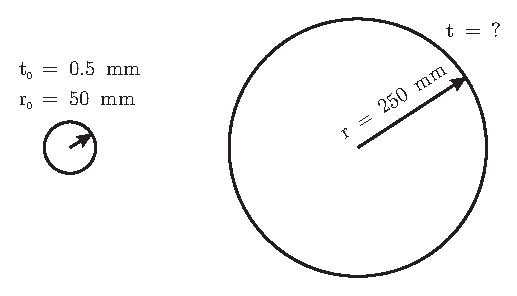
\includegraphics{balloon_soln_a.eps}
\end{figure}
\begin{figure}[h]
\centering
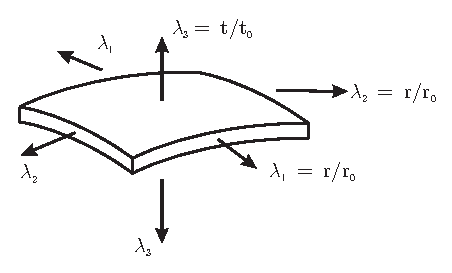
\includegraphics{balloon_soln_b.eps}
\end{figure}

As illustrated, the three principle stretches are
\begin{gather*}
\lambda = \lambda_1 = \lambda_2 = \frac{r}{r_0}\\
\lambda_3 = \frac{t}{t_0}
\end{gather*}
and they are related through the incompressibility condition
\begin{equation*}
\lambda_1 \lambda_2 \lambda_3 = 1
\end{equation*}
Combining and rearranging the above relations gives
\begin{gather*}
\lambda_3 = \lambda^{-2}\\
\frac{t}{t_0} = \left(\frac{r}{r_0}\right)^{-2}\\
t = t_0\left(\frac{r_0}{r}\right)^2 = 0.02\, \text{mm}
\end{gather*}

\item The  free body diagram for the thin walled pressure vessel
is shown below, and from it we can derive the pressure/stress
relation.
\begin{figure}[h]
\centering
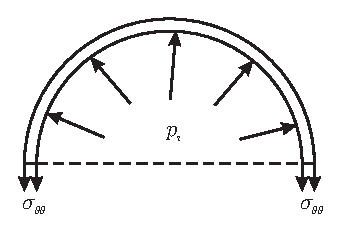
\includegraphics{balloon_soln_c.eps}
\end{figure}
\begin{gather}
\sigma_{\theta\theta} (2\pi r t) = \pi r^2 p_i \nonumber\\
\sigma_{\theta\theta} (2 t) =  r p_i \nonumber\\
\sigma_{\theta\theta} = \frac{ p_i r}{2t} \label{eqn1z}
\end{gather}
The constitutive relation for a neo-Hookean material is
\begin{equation*}
\sigma_i = \mu(\lambda_i^2 - p)
\end{equation*}
Using the boundary condition $\sigma_3 = 0$, we can solve for the
arbitrary pressure $p$
\begin{equation*}
0 = \mu(\lambda_3^2 - p) \quad \Longrightarrow \quad p = \lambda_3^2
= \lambda^{-4}
\end{equation*}
and hence
\begin{equation}
\sigma_{\theta\theta} = \mu(\lambda^2 - \lambda^{-4}) \label{eqn2}
\end{equation}
Substituting \eqref{eqn2} into \eqref{eqn1z} we get
\begin{equation}
p_i = 2 \frac{t}{r}\mu(\lambda^2 - \lambda^{-4})
\end{equation}
or
\begin{align}
p_i &= 2\mu  \frac{t_0}{r_0} \left( \frac{r_0}{r} \right)
\left(\frac{t}{t_0}\right)(\lambda^2 -
\lambda^{-4}) \nonumber\\
p_i &= 2\mu  \frac{t_0}{r_0}\,\lambda^{-1} \lambda^{-2} (\lambda^2
- \lambda^{-4}) \nonumber\\
\Longrightarrow \quad &\boxed{p_i = 2\mu
\frac{t_0}{r_0}(\lambda^{-1} - \lambda^{-7})}\label{eqn4}
\end{align}
\begin{figure}[h]
\centering
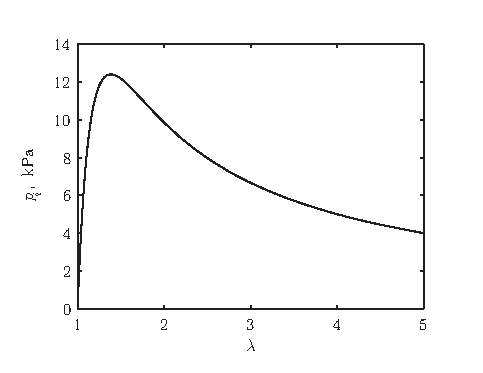
\includegraphics{balloon_soln_d.eps}
\end{figure}

\item For a maximum
\begin{gather*}
\frac{dp_i}{d\lambda} = 2\mu \frac{t_0}{r_0}\left(-\lambda^{-2} +
7\lambda^{-8} \right) = 0\\
\left(-\lambda^{-2} + 7\lambda^{-8} \right) = 0\\
7\lambda^{-8} = \lambda^{-2}\\
\lambda^{-6} = 1/7\\
\lambda = 1.3831
\end{gather*}
Using this stretch in \eqref{eqn4}
\begin{gather*}
p_{i,\text{max}} = 2 \,(1\times10^6) \left(\frac{0.5}{50}\right)
(1.3831^{-1} - 1.3831^{-7})\\
\boxed{p_{i,\text{max}} = 12.4\,\text{kPa}}
\end{gather*}

\item At the final inflation diameter, we have $\lambda=5$, and
using this in \eqref{eqn4}
\begin{gather*}
p_{i,\text{final}} = 2 \,(1\times10^6) \left(\frac{0.5}{50}\right)
(5^{-1} - 5^{-7})\\
\boxed{p_{i,\text{final}} = 4\,\text{kPa}}
\end{gather*}

\end{enumerate}
\end{document}
